% =============================================================================
%  Sanen Kinsen Hiroku — wraparound paperback cover (cover_final_5)
%
%  Layout (left-to-right, designer's spread):
%     [ back cover (6 in) ][ spine (0.367 in) ][ front cover (6 in) ]
%
%  Total trim: 12.367 in × 9.25 in. Spine width matches the prior
%  cover_final_5 print dimensions (book is ~55 pages, so the spine is
%  intentionally thin).
%
%  Back cover reserves a 2in × 1.2in barcode area in the lower-right
%  per Amazon KDP / IngramSpark requirements; the colophon block is
%  shifted left so it doesn't collide.
%
%  Compile with XeLaTeX. Uses a single TikZ canvas with x=1in/y=1in so
%  all coordinates can be read as inches from the page's lower-left
%  corner.
% =============================================================================

\documentclass[10pt]{article}

\usepackage[
  paperwidth=12.367in, paperheight=9.25in,
  margin=0pt
]{geometry}

\usepackage{fontspec}
\setmainfont{NotoSerif}[
  Path={/Users/grob/Library/TinyTeX/texmf-dist/fonts/truetype/google/noto/},
  Extension=.ttf,
  UprightFont=*-Regular,
  BoldFont=*-Bold,
  ItalicFont=*-Italic,
  BoldItalicFont=*-BoldItalic,
]
\IfFontExistsTF{Noto Serif CJK JP}{%
  \newfontfamily\japanesefont{Noto Serif CJK JP}[AutoFakeBold=2.5]%
}{%
  \newfontfamily\japanesefont{Hiragino Mincho ProN}[AutoFakeBold=2.5]%
}
\newcommand{\jp}[1]{{\japanesefont #1}}

\usepackage{tikz}
\usetikzlibrary{calc}
\usepackage{xcolor}
\usepackage{graphicx}

\definecolor{coverink}{HTML}{931A1D}
\definecolor{coverpaper}{HTML}{F4EBD3}
\definecolor{coverwarm}{HTML}{2B1612}

\pagestyle{empty}
\setlength{\parindent}{0pt}
\setlength{\fboxsep}{0pt}
\setlength{\topskip}{0pt}
\setlength{\parskip}{0pt}

\newcommand{\diaorn}{%
  \tikz[baseline=-0.5ex]\fill[coverink, rotate=45] (-1.4pt,-1.4pt) rectangle (1.4pt,1.4pt);%
}

\begin{document}
\noindent
\begin{tikzpicture}[x=1in, y=1in,
                    every node/.style={inner sep=0pt, outer sep=0pt}]

  % Page bounds: (0,0) bottom-left to (12.5, 9.25) top-right.
  % Force the picture to span the full page so margins of 0 are honored.
  \useasboundingbox (0,0) rectangle (12.367, 9.25);

  %------------------------------------------------------------------
  % Background paper + spine band (spine is 0.367 in wide — thin,
  % proportional to the book's 55-page bulk)
  %------------------------------------------------------------------
  \fill[coverpaper] (0, 0) rectangle (12.367, 9.25);
  \fill[coverink]   (6.0, 0) rectangle (6.367, 9.25);

  %==================================================================
  %  SPINE  (x in [6.0, 6.367])  — thin, matched to book bulk
  %==================================================================
  \node[rotate=-90, white, font=\fontsize{14}{16}\bfseries\selectfont]
    at (6.1835, 7.0) {\jp{三猿金泉秘録}};
  \node[rotate=-90, white, font=\itshape\small]
    at (6.1835, 4.0) {Sanen Kinsen Hiroku};

  % small white seal mark at base of spine
  \draw[white, line width=0.25pt] (6.1835, 0.45) circle [radius=2.5pt];

  %==================================================================
  %  FRONT COVER  (x in [6.367, 12.367], 6 inches wide)
  %  Local origin: (6.367, 0). Inner coords are (lx, y).
  %==================================================================

  % Top horizontal rule
  \draw[coverink, line width=0.6pt] (6.367+0.55, 8.55) -- (6.367+5.45, 8.55);

  % Japanese title
  \node[coverink, font=\fontsize{42}{48}\bfseries\selectfont]
    at (6.367+3, 7.85) {\jp{三猿金泉秘録}};

  % Italic romanization
  \node[coverink, font=\fontsize{20}{24}\itshape\selectfont]
    at (6.367+3, 7.05) {Sanen Kinsen Hiroku};

  % Lower divider with diamond at center
  \draw[coverink, line width=0.4pt] (6.367+0.85, 6.65) -- (6.367+2.85, 6.65);
  \draw[coverink, line width=0.4pt] (6.367+3.15, 6.65) -- (6.367+5.15, 6.65);
  \node at (6.367+3, 6.65) {\diaorn};

  % Radial diagram (height-limited so it doesn't intrude on title/subtitle)
  \node at (6.367+3, 4.45)
    {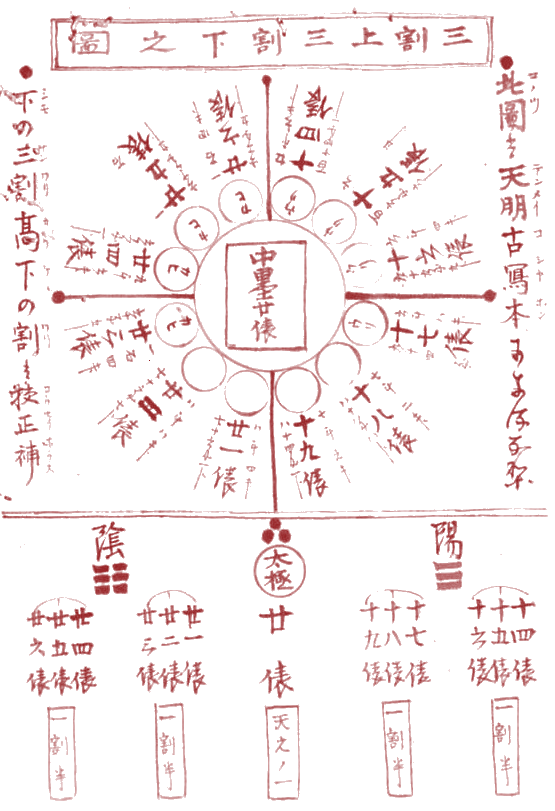
\includegraphics[height=4.3in]
      {../diagrams/diagram_grand_chart_red.png}};

  % Subtitle stack
  \node[coverink, font=\fontsize{17}{22}\selectfont]
    at (6.367+3, 2.00) {Three Monkeys Gold Spring};
  \node[coverink, font=\fontsize{17}{22}\selectfont]
    at (6.367+3, 1.70) {Secret Record};

  \node[coverink, font=\itshape]
    at (6.367+3, 1.32) {A Secret Record on the Art of};
  \node[coverink, font=\itshape]
    at (6.367+3, 1.12) {Rice Market Speculation};
  \node[coverink, font=\small]
    at (6.367+3, 0.88) {from the Edo Period of Japan};

  % Authors block divider
  \draw[coverink, line width=0.3pt] (6.367+0.85, 0.72) -- (6.367+5.15, 0.72);

  \node[coverink, font=\small]
    at (6.367+3, 0.55) {\jp{牛田権三郎}\hspace{1ex}Ushida Gonzaburō};
  \node[coverink, font=\small]
    at (6.367+3, 0.37) {\jp{鳴川猛之助}\hspace{1ex}Narukawa Takenosuke};

  \node[coverink, font=\footnotesize]
    at (6.367+3, 0.18) {Edited and produced by Zach Booth};

  %==================================================================
  %  BACK COVER  (x in [0, 6.0], 6 inches wide)
  %==================================================================

  % Top decorative ornament — small three-dot triangle above the rule
  \fill[coverink] (3 - 0.06, 8.62) circle [radius=1.4pt];
  \fill[coverink] (3 + 0.06, 8.62) circle [radius=1.4pt];
  \fill[coverink] (3,         8.55) circle [radius=1.4pt];

  % Top horizontal rule with diamond at center
  \draw[coverink, line width=0.4pt] (1.05, 8.40) -- (2.85, 8.40);
  \draw[coverink, line width=0.4pt] (3.15, 8.40) -- (4.95, 8.40);
  \node at (3, 8.40) {\diaorn};

  % Paragraph 1
  \node[coverink, text width=3.6in, align=center, font=\small,
        anchor=north]
    at (3, 8.10)
    {The Sanen Kinsen Hiroku is one of the most celebrated texts in
     the history of Japanese market speculation. Composed around 1755
     by Ushida Gonzaburō, an Osaka Dōjima trader, it belongs to a
     genre of secret transmission texts that circulated among
     Edo-period trading houses.};

  \node at (3, 6.50) {\diaorn};

  % Paragraph 2
  \node[coverink, text width=3.6in, align=center, font=\small,
        anchor=north]
    at (3, 6.30)
    {The title alludes to the proverb of the three monkeys --- ``see
     no evil, hear no evil, speak no evil'' --- reinterpreted as a
     warning: do not be swayed by what you see others doing, what you
     hear as rumor, or what you say in haste. Instead, observe the
     deeper patterns.};

  \node at (3, 4.50) {\diaorn};

  % Paragraph 3
  \node[coverink, text width=3.6in, align=center, font=\small,
        anchor=north]
    at (3, 4.30)
    {This is the first English translation of the actual Sanen Kinsen
     Hiroku, made directly from the 1851 manuscript held at Kyoto
     University.};

  % Taikyoku seal: three dots above + circle with 太極 inside
  \fill[coverink] (3 - 0.10, 2.30 + 0.55) circle [radius=0.04in];
  \fill[coverink] (3 + 0.10, 2.30 + 0.55) circle [radius=0.04in];
  \fill[coverink] (3,         2.30 + 0.42) circle [radius=0.04in];
  \draw[coverink, line width=0.8pt] (3, 2.30) circle [radius=0.32in];
  \node[coverink, font=\large\bfseries] at (3, 2.30) {\jp{太極}};

  % Bottom rule + colophon, shifted to the left half so the lower-right
  % can host the printer's barcode (KDP / IngramSpark requirement)
  \draw[coverink, line width=0.3pt] (0.4, 1.05) -- (2.95, 1.05);

  \node[coverwarm, font=\small]
    at (1.675, 0.85) {ISBN 979-8-254-10079-9};
  \node[coverwarm, font=\footnotesize\itshape, text width=2.5in,
        align=center]
    at (1.675, 0.60) {English translation © 2026 Zach Booth\\
                      Manuscript courtesy of the Main Library,
                      Kyoto University};

  % Barcode placeholder — 2 in × 1.2 in, lower-right of back cover.
  % Standard ISBN/EAN-13 barcode fits a 1.5×1 in active area; the
  % 2×1.2 in box gives the printer the recommended quiet zone.
  % Rendered as a thin outline so the print pipeline can overlay
  % the actual barcode image at production time.
  \draw[coverink!40, line width=0.3pt, dashed]
    (3.5, 0.30) rectangle (5.5, 1.50);
  \node[coverink!50, font=\footnotesize\itshape] at (4.5, 0.90)
    {ISBN barcode};

\end{tikzpicture}%
\end{document}
